\chapter{Project Context}

\section{Introduction}
This chapter presents the host company, exploring its history, sectors of
activity, and client portfolio. It also examines the project context by
analyzing the existing situation, identifying its limitations, and proposing
a solution to enhance the firm's operations. Finally, it describes the
dataset used to build the system's knowledge base.

\section{Host Company Presentation}
This section introduces the host company, Jade Advisory, drawing on publicly available sources.

\subsection{Jade Advisory Presentation}
Jade Advisory \cite{WJade} is a consulting firm specializing in infrastructure
finance and Public-Private Partnerships. Established in 2019 in Tunis, the
company later opened offices in London (2020) and France (2024). With over
50 projects across Africa, the MENA region, and Europe, Jade Advisory brings
together experts in finance, transport economics, and infrastructure planning.

The firm provides technical advice to help clients develop cost-effective,
sustainable, and innovative solutions, guiding them through all stages of a
project's lifecycle. Its services include advisory, training programs, project
management, and infrastructure consulting focused on Public-Private Partnerships
(PPP). Essentially, Jade Advisory supports public and private entities in
structuring, evaluating, and managing complex projects, assessing financial
viability and risks, and facilitating partnerships to streamline implementation.
Delivering successful and valuable outcomes for every client remains its top
priority.

\subsection{Sectors of Activity}
Their specialization in Public-Private Partnerships enables them to deliver
high-quality reports and strategic advice to both private sector actors and
government agencies. Jade Advisory operates across several key sectors,
including water management, municipal services, social infrastructure,
transport, agriculture, and other infrastructure-related fields.

\subsection{Clients of Jade Advisory}
Due to its experience, reliability, and commitment to delivering high-quality
advisory services, Jade Advisory has built a strong and trusted client base,
as presented in \textbf{Figure~\ref{fig:jade_clients}}. Over the years, the company
has collaborated with public institutions, government agencies, and private
sector organizations across Africa, the MENA region, and Europe, supporting
the planning, structuring, and implementation of infrastructure and
Public-Private Partnership projects.

\begin{figure}[H]
    \centering
    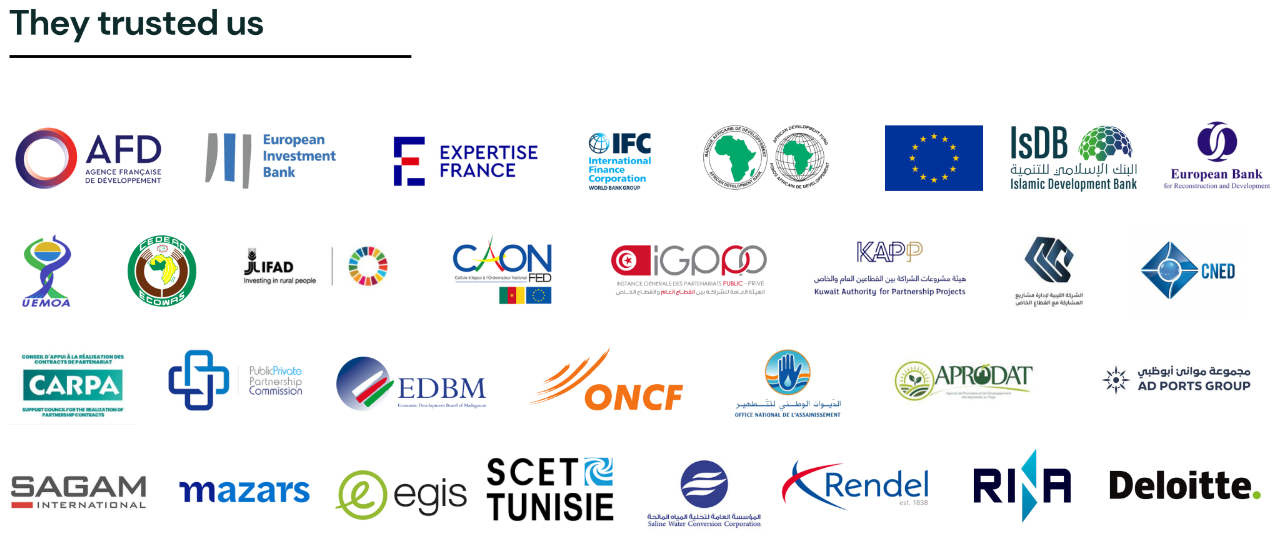
\includegraphics[width=1\linewidth]{JadeClients.png}
    \caption{Clients of Jade Advisory}
    \label{fig:jade_clients}
\end{figure}

\section{Project Presentation}
In this section we will discuss the existing situation, identify its problems,
and offer solutions to improve it and support the company's success.

\subsection{Study of The Existing Solution}
The document library of Jade Advisory is growing significantly with every new
project, making manual knowledge retrieval for guidance and learning
increasingly difficult. As a result, there is a growing need for a smart
knowledge retrieval and document management solution to help teams access
relevant insights efficiently.

Recognizing the challenges that came from exponential data growth, software
companies such as OpenAI, IBM and Microsoft made it their mission to develop
intelligent solutions, including AI assistants integrated into a knowledge
base, or systems where documents can be provided as input and questions asked
directly. These solutions make it easier for organizations to extract, manage
and use knowledge more efficiently.

\textbf{Table~\ref{tab:tools_definition}} presents a brief description of some
existing intelligent solutions.

\begin{table}[H]
    \centering
    \caption{Existing AI and Knowledge Management Tools}
    \renewcommand{\arraystretch}{1.2}
    \begin{tabular}{|l|p{10cm}|}
        \hline
        \textbf{Tool} & \textbf{Definition} \\
        \hline
        Microsoft Copilot \cite{copilot} & AI assistant integrated into Microsoft 365
        and SharePoint. Users can ask questions in natural language and retrieve
        answers directly from stored documents in SharePoint. \\
        \hline
        IBM Watson \cite{ibmwatson} & AI-powered knowledge management platform with
        natural language querying, document analysis, and enterprise security.
        Helps extract insights from large repositories. \\
        \hline
        Notion AI \cite{notionai} & AI assistant within Notion that summarizes notes,
        searches information, and generates content. Limited for versioned project
        documents. \\
        \hline
        Duet AI \cite{duetai} & Google's AI assistant in Docs, Sheets, and Drive.
        Summarizes documents, answers questions, and assists content creation.
        Data is cloud-stored. \\
        \hline
    \end{tabular}
    \label{tab:tools_definition}
\end{table}

While these tools offer advanced capabilities for knowledge management, it is
important to evaluate how well they meet the specific needs of Jade Advisory.

\subsection{Criticism of The Existing Solution}
To better understand the limitations of these tools, the following criteria
are used to evaluate their performance in the context of the company.

\begin{itemize}
    \item \textbf{Knowledge Capture:} Ability of the tool to store, organize,
    and retrieve project knowledge and lessons learned effectively.
    \item \textbf{Domain Specificity:} How well the tool handles content
    specific to the organization's domain or industry.
    \item \textbf{Data Privacy:} Indicates whether the tool keeps documents
    accessible only to the company, or if data is also stored or accessible
    by cloud providers.
    \item \textbf{Customization:} The extent to which the tool allows
    customization for workflows, document structures, and AI responses.
    \item \textbf{Dependency:} The degree to which the tool relies on
    external ecosystems or platforms.
    \item \textbf{Pricing:} Cost of the tool, including licensing,
    subscription, and any hidden fees.
\end{itemize}

\textbf{Table~\ref{tab:tools_comparison_explained}} presents a structured comparison
of the existing AI tools based on the criteria defined above.

\begin{table}[H]
\centering
\caption{Comparison of Existing AI-Based Solutions}
\label{tab:tools_comparison_explained}
\renewcommand{\arraystretch}{1.3}
\begin{tabular}{|>{\raggedright\arraybackslash}p{2.8cm}
|>{\raggedright\arraybackslash}p{3cm}
|>{\raggedright\arraybackslash}p{3cm}
|>{\raggedright\arraybackslash}p{3cm}
|>{\raggedright\arraybackslash}p{3cm}|}
\hline
\textbf{Criteria} & \textbf{Microsoft Copilot} & \textbf{IBM Watson}
& \textbf{Notion AI} & \textbf{Duet AI} \\
\hline
Knowledge Capture & Can search and summarize SharePoint documents &
Extract information from large datasets & Summarizes notes but struggles
with many files & Summarizes Google Docs and Sheets \\
\hline
Domain Specificity & Generic, not adapted to Jade Advisory &
Customizable for specific industries & Limited understanding of
specialized documents & Mainly designed for common office documents \\
\hline
Data Privacy & Data stored in Microsoft Cloud with some control &
Strong enterprise-level security & Stored in Notion Cloud with some
privacy concerns & Data stored in Google Cloud services \\
\hline
Customization & Limited AI customization & Highly customizable
workflows and analysis & Basic customization features &
Very limited customization \\
\hline
Dependency & Strong dependence on Microsoft 365 ecosystem &
Depends on IBM Cloud infrastructure & Fully dependent on the
Notion platform & Integrated into Google Workspace ecosystem \\
\hline
Pricing & High subscription cost & Expensive enterprise licensing &
Affordable for small teams & Expensive with Google Workspace \\
\hline
\end{tabular}
\end{table}

The comparison presented in \textbf{Table~\ref{tab:tools_comparison_explained}}
shows that the evaluated tools do not fully meet the needs of Jade Advisory.
They are either costly or not well adapted to specialized document management.

Moreover, most of them rely on external cloud infrastructures, which raises
serious data privacy concerns and limits the organization's control over
sensitive information. This dependency on third-party services may also
affect flexibility and long-term scalability, especially for internal
knowledge management systems. In addition, these tools are not specifically
designed for the complexity of Public-Private Partnerships (PPP) related
documents, which include legal, financial, and technical content.

Another important limitation is the lack of traceability in the generated
answers. Users cannot easily identify the original source of information,
such as the exact document or section, which is essential in a professional
consulting context where accuracy and verification are critical.

These limitations clearly highlight the need for a tailored solution that is
secure, efficient, and better adapted to the organization's requirements,
while ensuring better control, traceability, and relevance of the retrieved
information.

\section{Proposed Solution}
As a solution to the challenges identified in the existing knowledge
management system, this project proposes the development of a centralized,
intelligent document management system based on a Retrieval-Augmented
Generation (RAG) approach, named Ask-Jade.

This system will transform Jade Advisory's dispersed document library into
a structured and searchable knowledge base. By using advanced AI
technologies and modern data engineering practices, Ask-Jade will allow
team members to retrieve information quickly and accurately, answer queries
contextually, and access insights from past projects more efficiently.
Unlike the generic tools evaluated in the previous section, it is
specifically designed to handle the multilingual, multimodal, and
domain-specific nature of Jade Advisory's document corpus, ensuring that
all project documents, reports, meeting minutes, and legal files are
indexed in a single structured repository.

The proposed solution will also standardize document organization, indexing,
and metadata management, making it easier to locate, update, and reuse
knowledge across projects. Data privacy is ensured by keeping all documents
within the organization's infrastructure, giving the firm full control over
its sensitive project data.

In addition, Ask-Jade provides flexibility in response generation by
allowing users to choose between different Large Language Models (LLMs)
according to their needs. This enables users to adapt the system based on
the desired balance between response quality, speed, and cost, offering a
more personalized and efficient user experience.

For new employees, Ask-Jade will serve as a learning tool, providing fast
access to relevant project information and organizational practices.
Overall, this approach is designed to enhance productivity, reduce errors,
and improve decision-making, empowering Jade Advisory to make better use of
its institutional knowledge and ultimately supporting the firm's growth and
continued success.

%=============================================================
\section{Dataset Description}
\label{sec:dataset}
%=============================================================

The quality and diversity of the dataset directly impact the performance
of the Retrieval-Augmented Generation (RAG) system. This section presents
the document corpus used in this project, including its structure, formats,
and main processing challenges.

\subsection{Dataset Overview}

The dataset is composed of internal enterprise documents related to
Public-Private Partnership (PPP) projects and consulting activities. It
was collected from the organization's SharePoint platform and includes
various types of content such as reports, meeting minutes, operational
guides, and legal contracts written in English, French, and Arabic.

The corpus is heterogeneous, multilingual, and multimodal, combining
textual content, tables, and visual elements across multiple file formats,
mainly PDF, DOCX, and PPTX. Some PDF files are scanned and contain
non-selectable text and embedded images.

This diversity increases the complexity of information processing and
retrieval, as it requires different extraction strategies depending on
the structure, format, and content type of each document.

\textbf{Table~\ref{tab:doc_types}} presents the main content types identified
in the dataset.

\begin{table}[H]
\centering
\caption{Document types in the dataset}
\renewcommand{\arraystretch}{1.3}
\begin{tabular}{|l|p{6cm}|p{3cm}|}
\hline
\textbf{Document Type} & \textbf{Description} & \textbf{Content} \\
\hline
Meeting Minutes &
Discussions, decisions, and action items from meetings.
Semi-structured with text and simple tables. &
Text, Tables \\
\hline
Technical and Financial Reports &
Project progress, KPIs, and financial analysis. &
Text, Tables, Charts \\
\hline
Operational Guides and Manuals &
Internal procedures using structured instructions and diagrams. &
Text, Images, Charts \\
\hline
Contractual and Legal Documents &
Formal agreements organized into articles and clauses. &
Text \\
\hline
\end{tabular}
\label{tab:doc_types}
\end{table}

\textbf{Table~\ref{tab:content_types}} summarises the main content categories
included in the dataset.
\begin{table}[H]
\centering
\caption{Multimodal content types in the dataset}
\renewcommand{\arraystretch}{1.3}
\begin{tabular}{|l|p{5.5cm}|p{3cm}|}
\hline
\textbf{Content Type} & \textbf{Description} & \textbf{Format} \\
\hline
Text &
Narrative content including legal clauses and technical terminology
written in multiple languages. &
PDF, DOCX, PPTX \\
\hline
Tables &
Structured information such as budgets, KPIs, and schedules extracted
from reports. &
PDF, DOCX, PPTX \\
\hline
Images and Charts &
Visual elements such as diagrams, figures, and scanned content requiring
OCR and layout-aware parsing. &
PDF, PPTX \\
\hline
\end{tabular}
\label{tab:content_types}
\end{table}
\textbf{Figure~\ref{fig:dataset_example}} shows an example of a representative
document from the dataset, combining formatted text and table.
\begin{figure}[H]
\centering
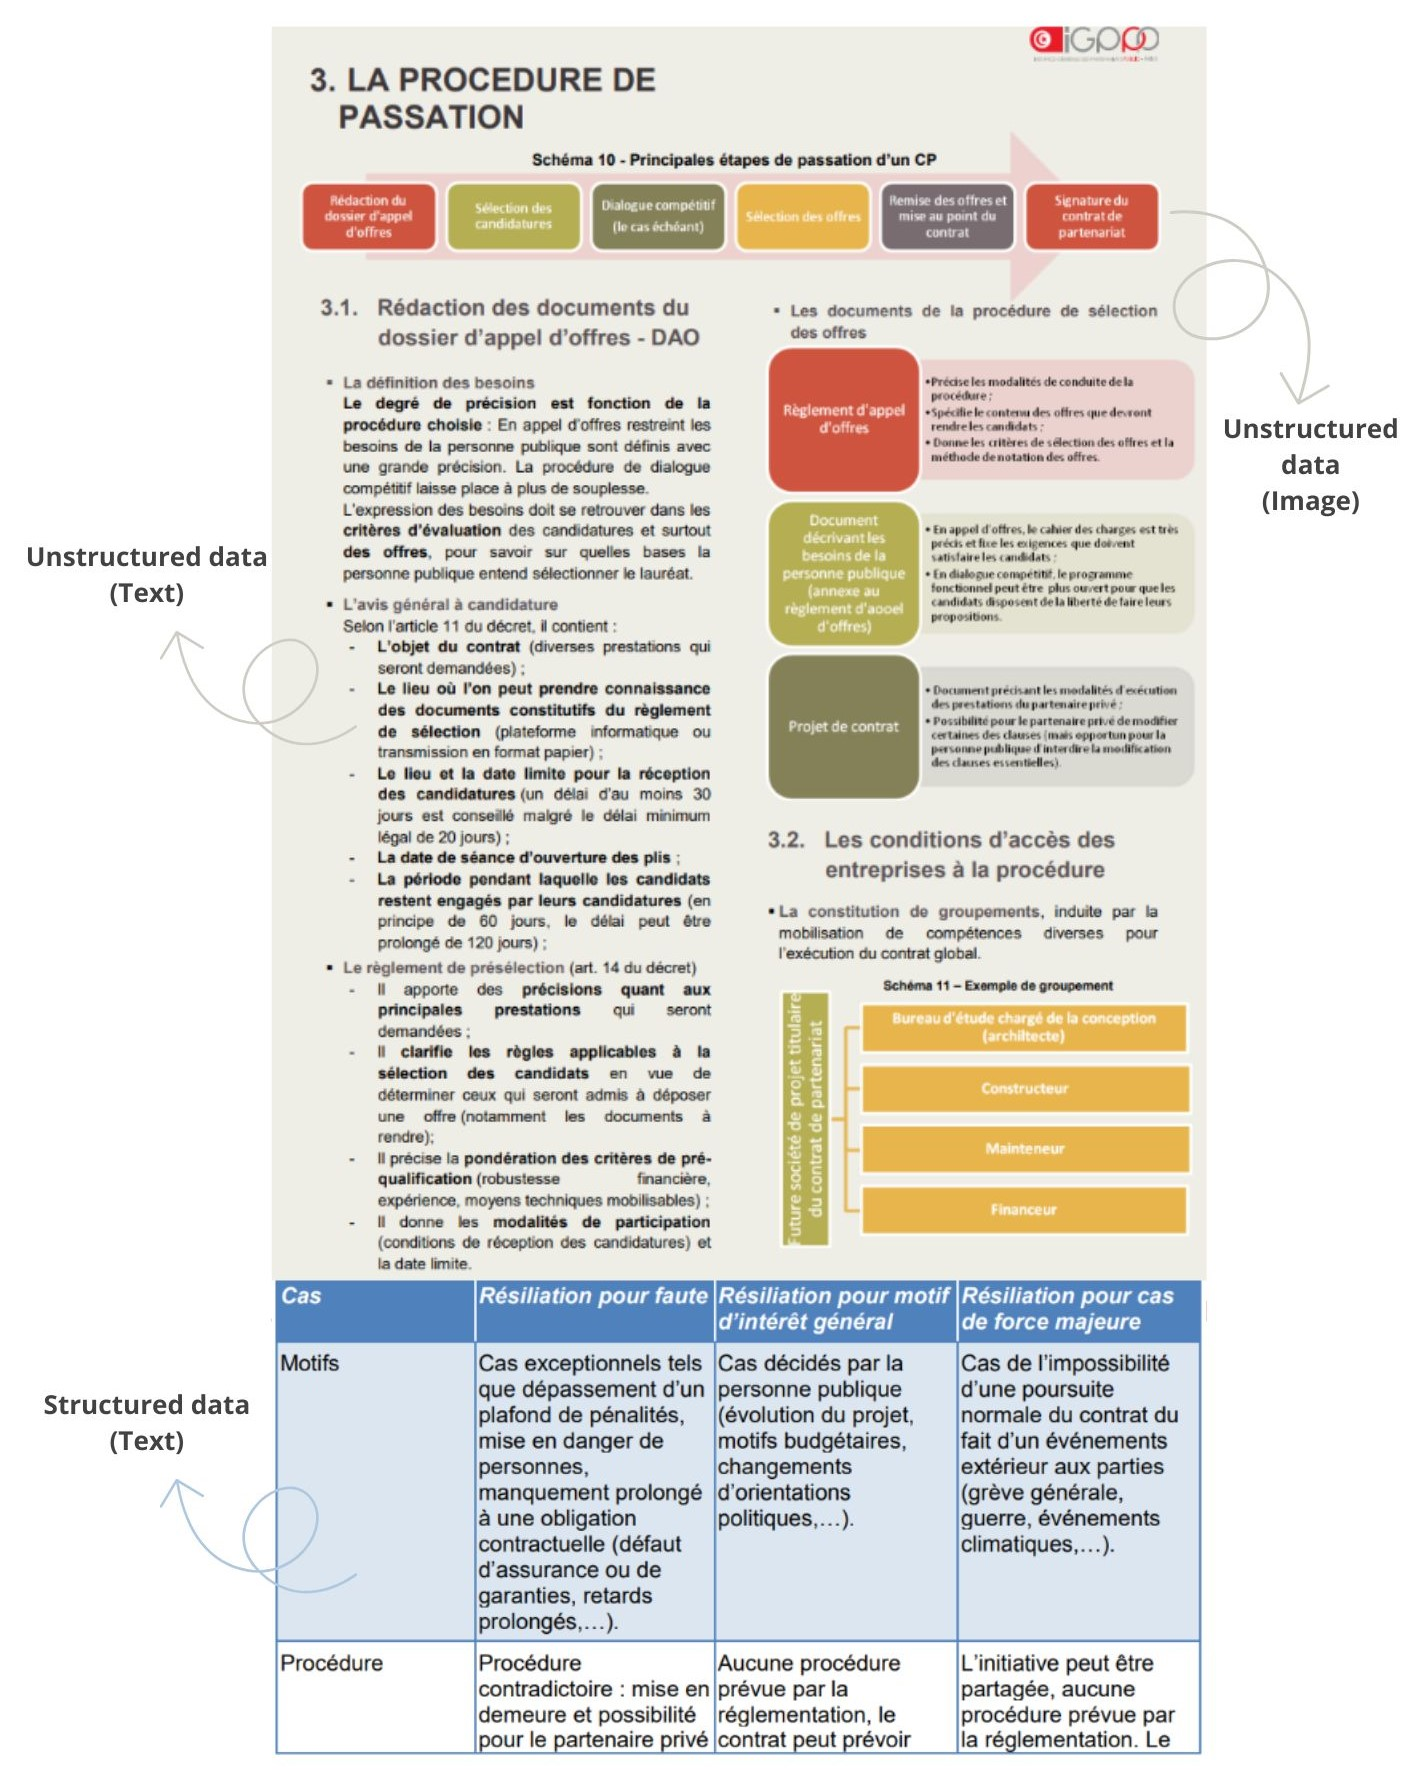
\includegraphics[width=0.5\textwidth]{data_jade.jpg}
\caption{Example of a document from the dataset}
\label{fig:dataset_example}
\end{figure}

\subsection{Technical Challenges and Design Implications}

The dataset introduces several challenges that directly influenced the
design of the proposed RAG pipeline.

\begin{itemize}
    \item \textbf{Heterogeneous file formats:}
    The dataset contains multiple file types, including PDF, DOCX, and
    PPTX. This requires a unified parsing strategy to ensure consistent
    and reliable document processing across all formats.

    \item \textbf{Multimodal structure:}
    Documents include a combination of textual content, tables, and visual
    elements such as figures and diagrams. This necessitates layout-aware
    extraction techniques capable of preserving structural and semantic
    relationships.

    \item \textbf{Scanned documents:}
    Some PDF files are image-based and do not contain selectable text.
    Optical Character Recognition (OCR) techniques are therefore required
    to extract and reconstruct textual information accurately.

    \item \textbf{Domain-specific terminology:}
    The corpus includes financial, legal, and technical vocabulary. This
    requires embedding models capable of capturing domain-specific semantics
    to improve retrieval accuracy.

    \item \textbf{Multilingual content:}
    The dataset contains documents written in Arabic, English, and French.
    This introduces challenges for cross-lingual retrieval and requires
    support for multilingual embeddings.
\end{itemize}

\section{Conclusion}
This chapter introduced Jade Advisory and evaluated existing knowledge 
management tools, revealing key limitations in terms of domain specificity, 
data privacy, and traceability. These shortcomings motivated the proposal 
of Ask-Jade, a RAG-based solution tailored to the organization's needs. 
The following chapter presents a structured needs analysis of the system, 
defining its requirements, actors, and conceptual models.